\begin{figure}[t]
\vspace*{-5ex}
\centering
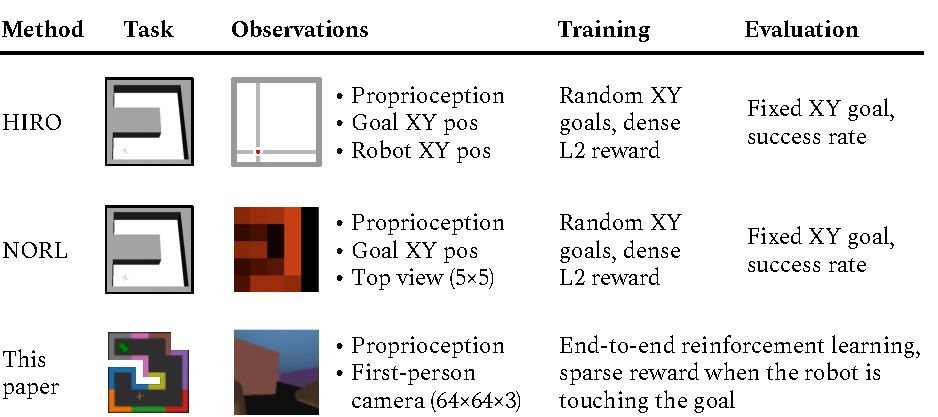
\includegraphics[width=\textwidth]{inputs/inputs}
\caption{
Comparison of Ant Mazes in the literature and this paper. 
HIRO \citep{nachum2018hiro} provided global XY coordinates of the goal and robot position to the agent and trained with dense rewards on uniformly sampled training goals. 
NORL \citep{nachum2018norl} replaced the robot XY position with a global top-down view of the environments, downsampled to 5$\times$5 pixels. 
In this paper, we tackle the more challenging problem of learning directly from an egocentric camera without global information provided to the agent, and only give a sparse reward for time steps where the robot is at the goal. 
To succeed at these tasks, an agent has to autonomously explore the environment and identify landmarks to localize itself and navigate the mazes.
}
\label{fig:inputs}
\end{figure}